\documentclass{article}

\usepackage{amsmath}
\usepackage{amssymb}
\usepackage{hyperref}
\usepackage{url}
\usepackage{graphicx}
\usepackage{geometry}
\usepackage{enumitem}
\usepackage{parskip}
\usepackage{chemfig}
\usepackage{pdfpages}
\usepackage{xcolor}
\usepackage{tikz}
\usepackage{fancybox}
\usepackage{makecell}
\usepackage{pgfplots}
\usepackage{soul}
\usepackage{ulem}
\usepackage{wrapfig}
\usepackage{subcaption}
\usepackage[T1]{fontenc}
\usepackage{esvect}
\usepackage{multirow}
\usetikzlibrary{arrows}
\usetikzlibrary{decorations.pathreplacing}
\pgfplotsset{compat=1.17}
\usepgfplotslibrary{statistics}
\definecolor{darkgray}{rgb}{0.2, 0.2, 0.2}

% === BIBLIOGRAPHY ===
\usepackage[utf8]{inputenc}
\usepackage{csquotes}
\usepackage[style=apa, backend=biber, doi=true, url=true]{biblatex}
\addbibresource{ref.bib}
\DeclareFieldFormat[article]{volume}{\textbf{#1}}
\DeclareFieldFormat[article]{journaltitle}{\textit{#1}}
% ====================
 
\geometry{
    a4paper,
    total={170mm, 257mm},
    left=20mm,
    top=20mm
}

\hypersetup{
    colorlinks=true,
    linkcolor=black,
    urlcolor=blue,
    pdftitle={Report SW05 - EnCheBio}
}

\newcommand{\figbox}[1]{ 
    \begin{figure*}[ht!]        
        \begin{center}            
            \fbox{#1}        
        \end{center}    
    \end{figure*}
}

\newcommand{\wrapfill}{
    \par
    \ifnum \value{WF@wrappedlines} > 0
        \addtocounter{WF@wrappedlines}{-1}%
        \null\vspace{
            \arabic{WF@wrappedlines}
            \baselineskip
        }
        \WFclear
    \fi
    \phantom{}
}

\newcommand{\cfig}[1]{%
  \begin{figure*}[ht!]%
    \centering%
    #1%
  \end{figure*}%
}

\newcommand{\difference}{\,\backslash\,}
\newcommand{\rem}{\underline{Remark}: }
\newcommand{\nots}{\underline{Notation}: }
\newcommand{\prf}{\underline{Proof}: }
\newcommand{\exs}{\underline{Example}: }
\newcommand{\defs}{\underline{Definition}: }
\newcommand{\wrn}{\underline{Warning}: }
\newcommand{\sht}{\ |\ }
\newcommand{\pph}[1]{\paragraph{#1}\phantom{}\\}

% === TEXT ===
\title{\textbf{Practical 1 \\ Environmental chemistry and biology \\ HSLU, Semester 1}}
\author{Matteo Frongillo}

\begin{document}

\hypersetup{citecolor=black}

\begin{minipage}{0.7\textwidth}
    \vspace*{-.8cm} \hspace*{-0.3cm}
    
\includegraphics[width=.5\textwidth]{media/hslu-logo.png}
\end{minipage}

\vspace*{2cm}

\textbf{\huge Practical 1:}\\[.75cm]
\begin{center}
    \textbf{\huge Composting Parameters and}
    
    \textbf{\huge Plant Tolerance Test}\\[1cm]
    
    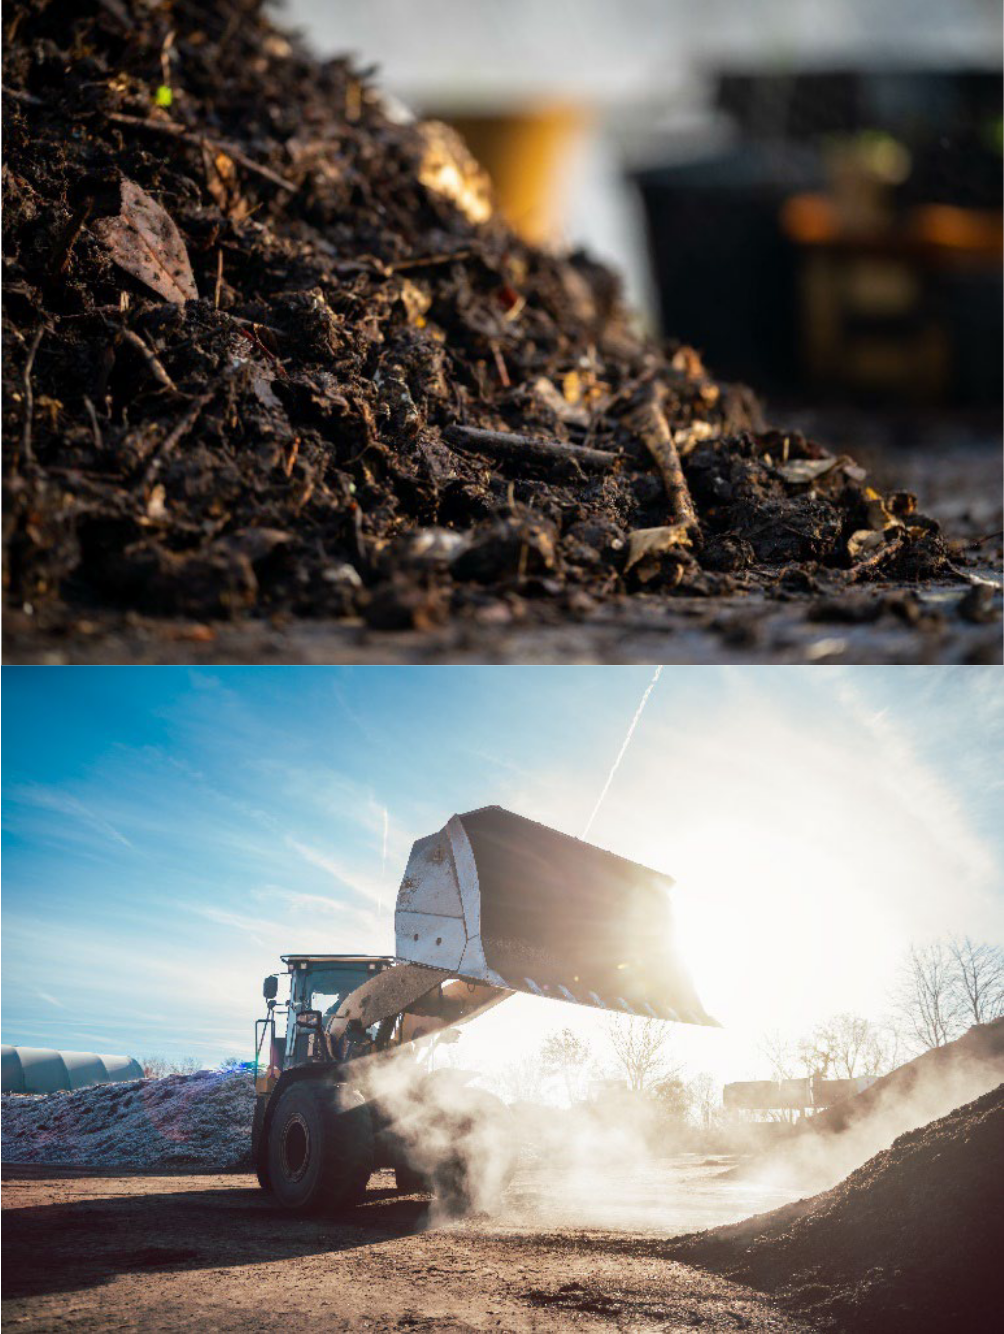
\includegraphics[width=0.6\textwidth]{media/front_practical1.png}\\
\end{center}

\vspace*{1cm}

\setlength{\intextsep}{0pt}%
\begin{wrapfigure}{r}{\textwidth}
    \textbf{\Large Environmental Chemistry and Biology HS2024\\[.5cm]
    \large Dr. Macarena San Martín Ruiz\\
    Lecturer}
    \vspace{-2.1cm}
\end{wrapfigure}

\phantom{}\\[-1cm]

\begin{flushright}
        \large
        \textbf{Team 4}\\
        Matteo Frongillo\\
        Ramadhan Nura\\
        Folagbade Popoola\\
        Jonathan Lawrence Boms\\
        Kron Xhemajli
\end{flushright}
\wrapfill

\tableofcontents
\pagebreak

\section{Composting parameters and plant tolerance test}
\subsection{Introduction}
This experiment focuses on understanding how different types of compost affect plant
growth. It aims to explore the chemical and physical interactions between compost and
plant systems. Gaining a better understanding of these processes is essential for
improving sustainable farming methods, making nutrients more available to plants, and
managing resources effectively in agriculture.

\subsection{Materials and methods}
For this experiment, six gardening pots, three buckets containing different types of 
compost, a containment box, and a sieve were provided.

A scale and a measuring cylinder were used to determine the mass of the compost types
(fresh, standard, and finished). The initial and final temperatures at the bottom of each
pot were measured using a probe thermometer. Subsequently, pH measurements were conducted on each type of compost, with the samples
dissolved in distilled water in a small beaker. Next, the composts were placed into different pots and divided into three distinct
groups: 50\% finished and 25\% finished compost, 50\% fresh and 25\% fresh compost, and
standard soil.

Finally, 15 seeds were carefully placed in each pot, and their growth and development
were closely monitored.
\vspace*{.6cm}

\begin{figure}[ht!]
    \begin{minipage}[b]{0.5\textwidth}
        \centering
        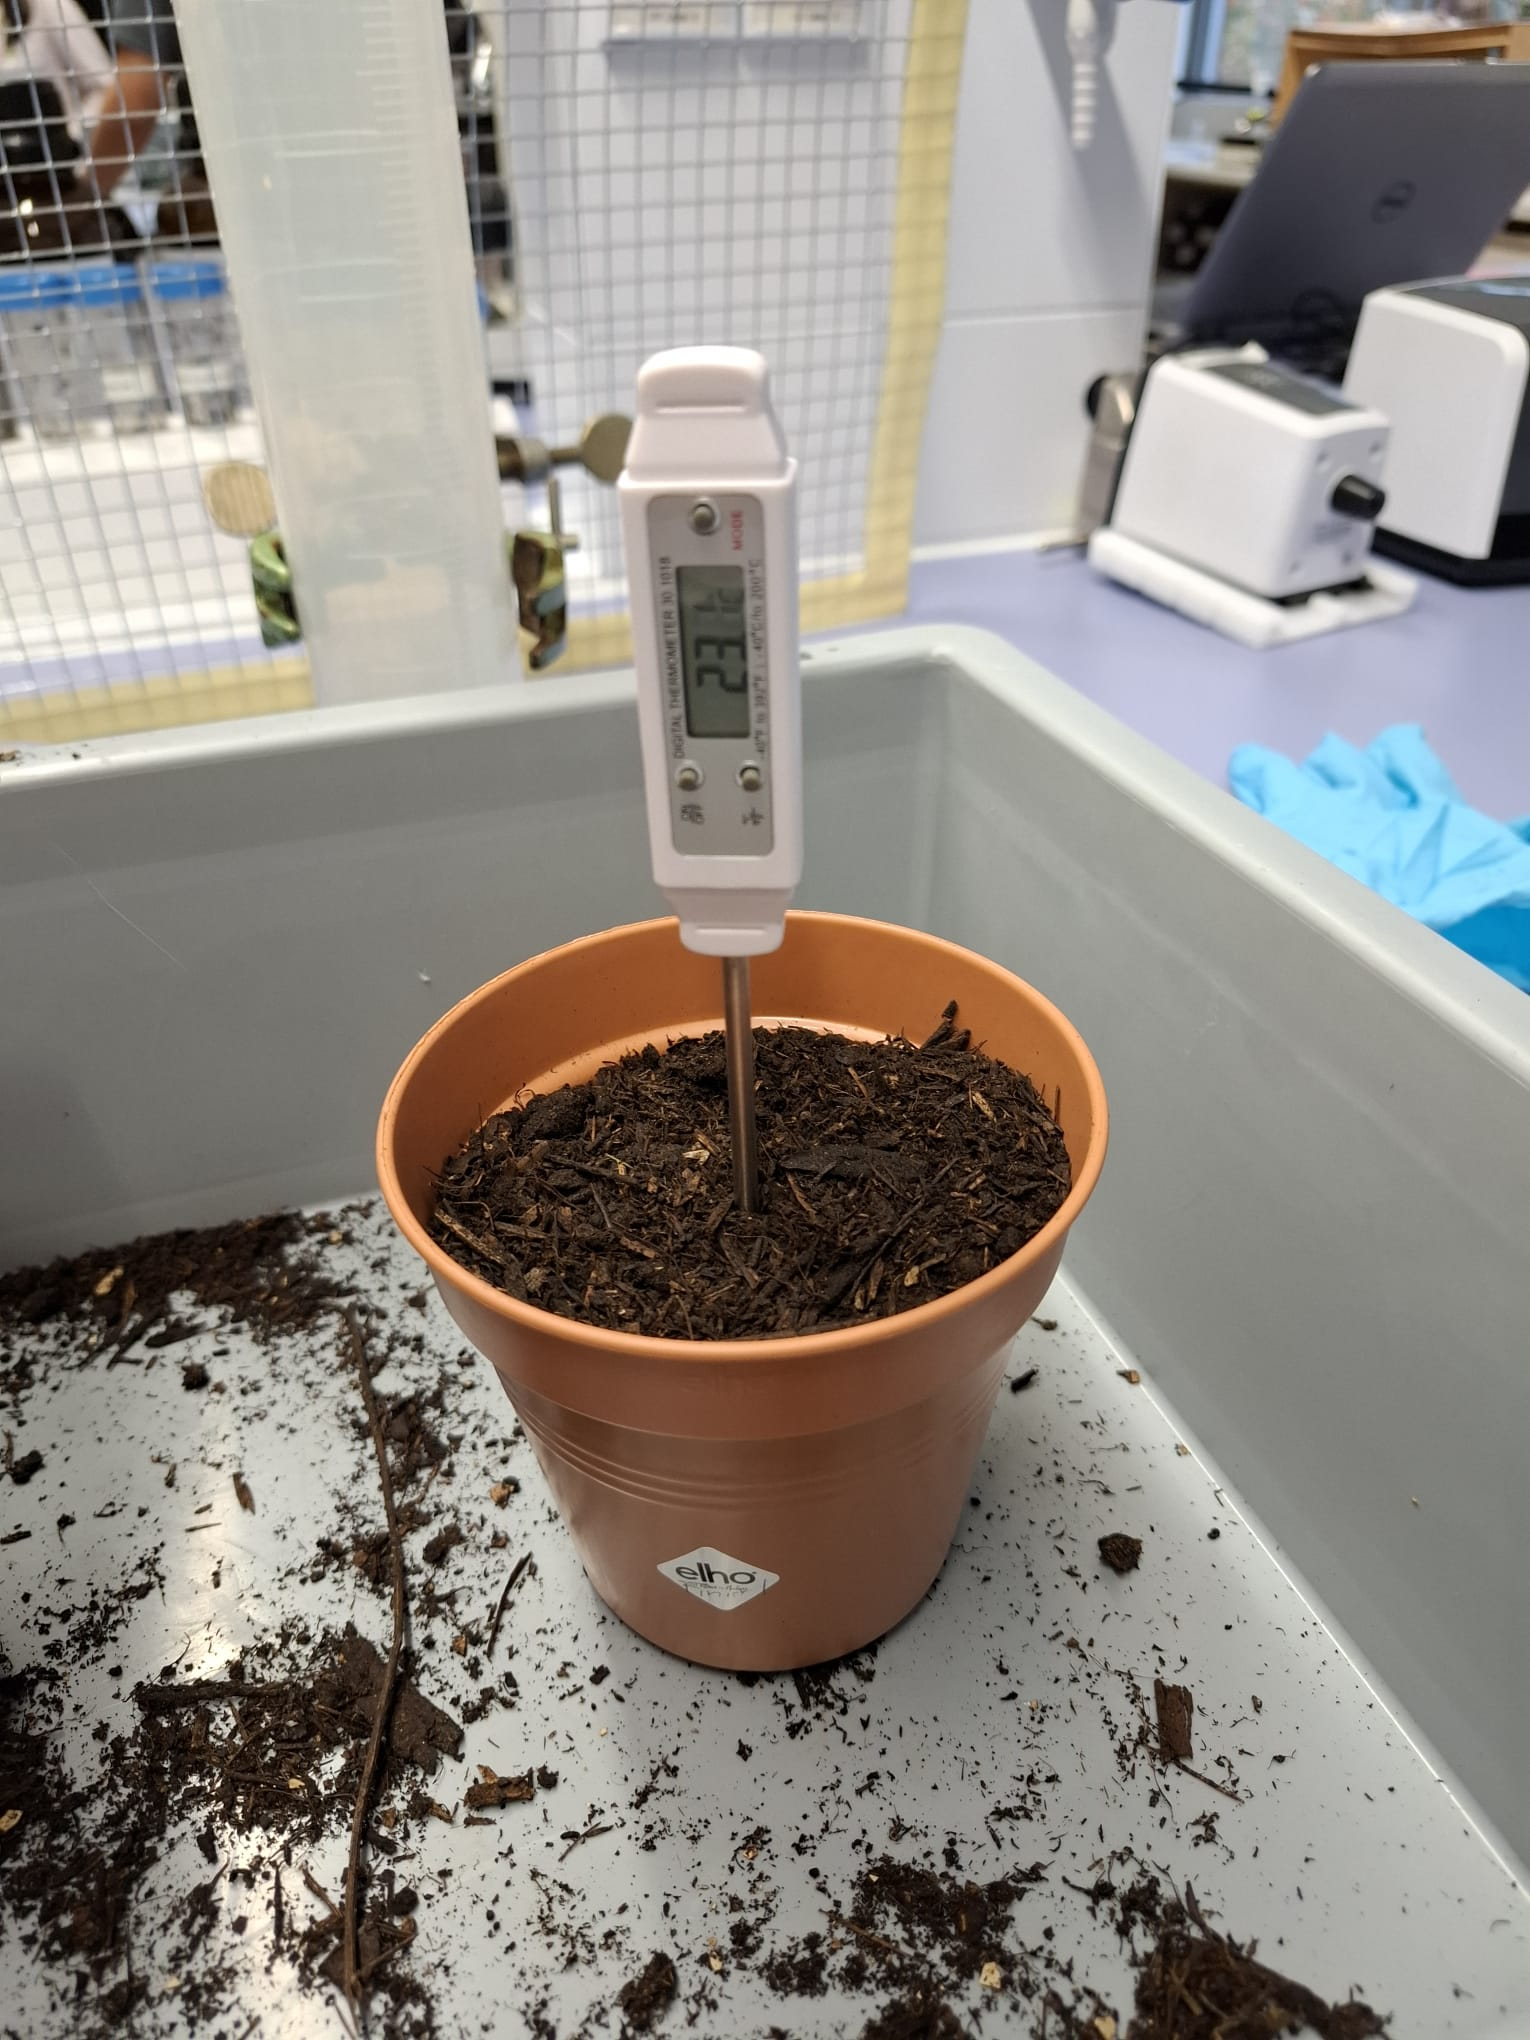
\includegraphics[width=.5\textwidth]{media/pot-temp.jpeg}
        \caption{Pot temperature}
    \end{minipage}%
    \hfill
    \begin{minipage}[b]{0.5\textwidth}
        \centering
        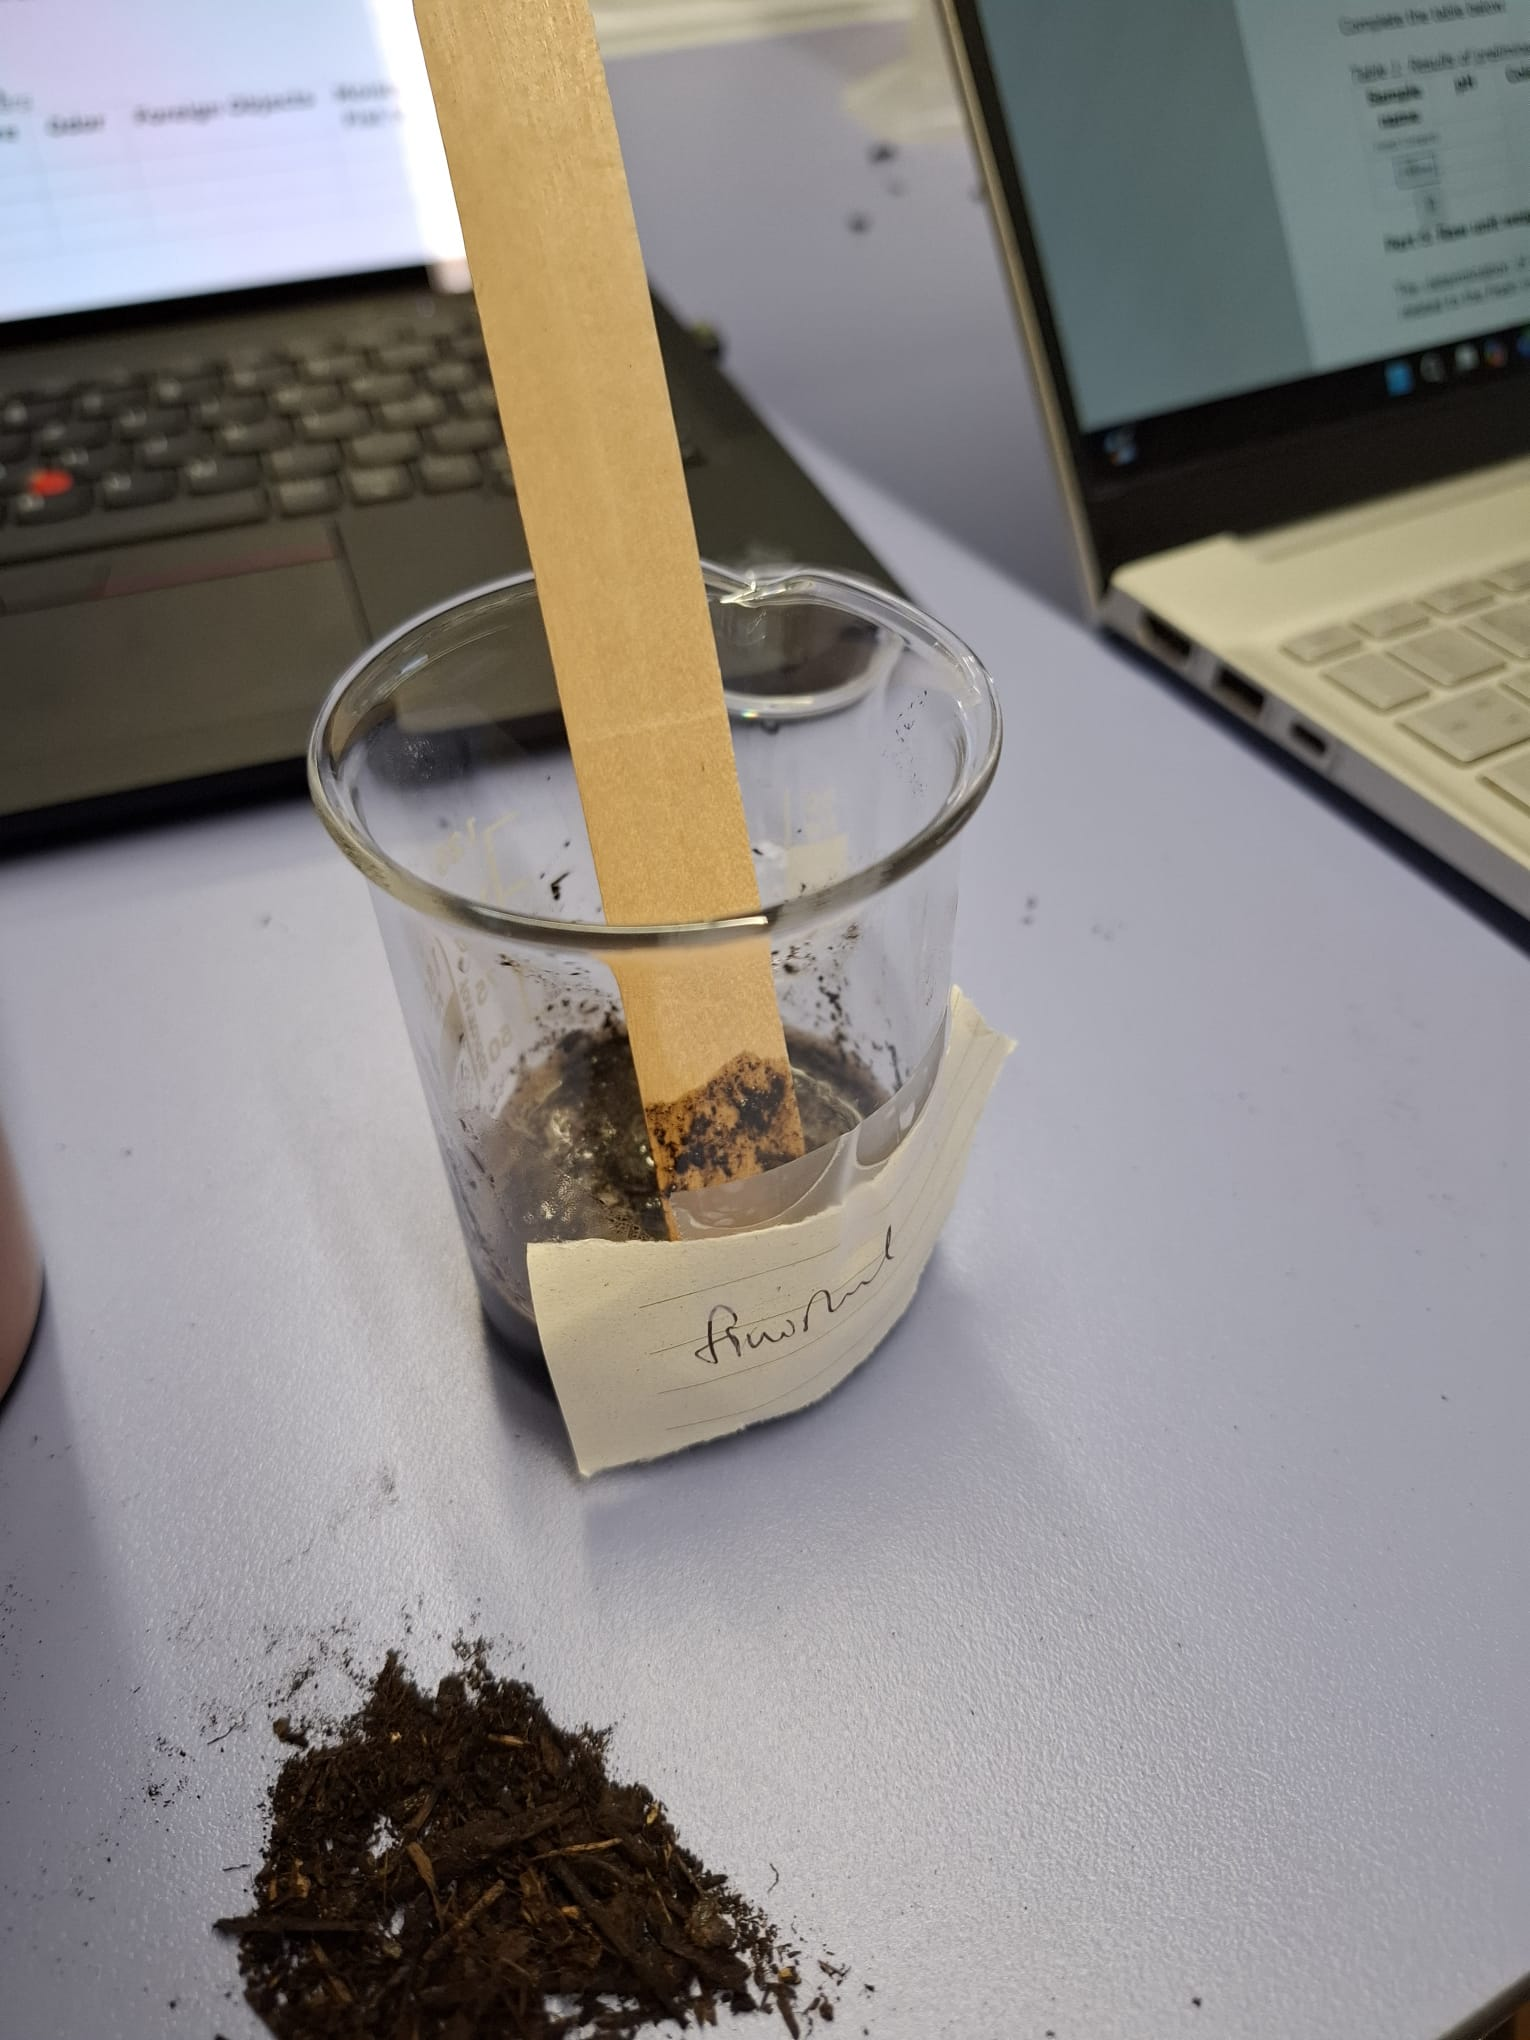
\includegraphics[width=.5\textwidth]{media/ph-mix.jpeg}
        \caption{Compost dissolution}
    \end{minipage}%
\end{figure}
\vspace*{1cm}

\begin{figure}[ht!]
    \begin{minipage}[b]{0.5\textwidth}
        \centering
        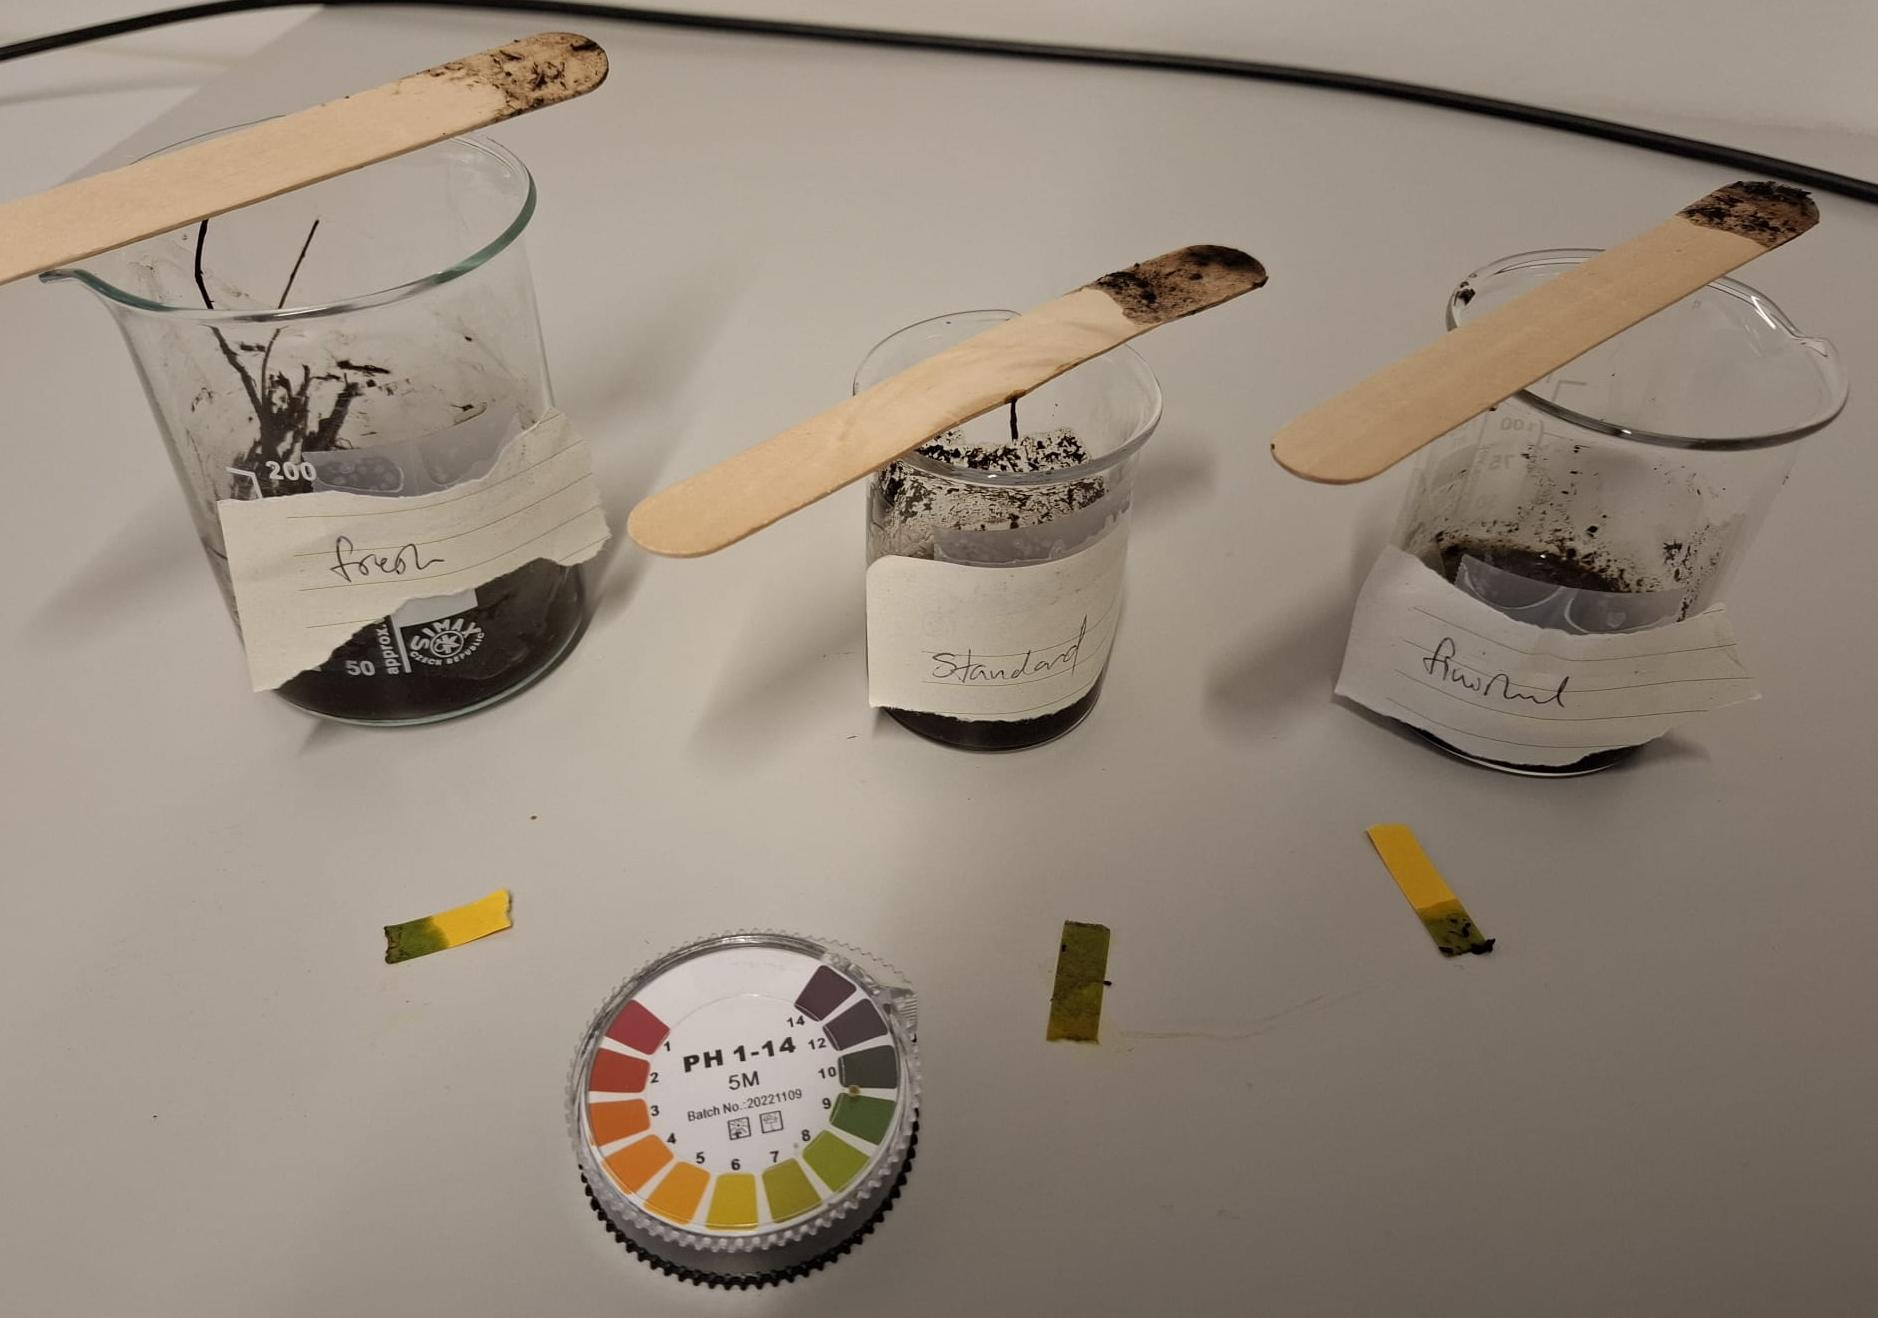
\includegraphics[width=\textwidth]{media/ph-results.jpeg}
        \caption{Compost pH results}
    \end{minipage}
    \hfill
    \begin{minipage}[b]{0.5\textwidth}
        \centering
        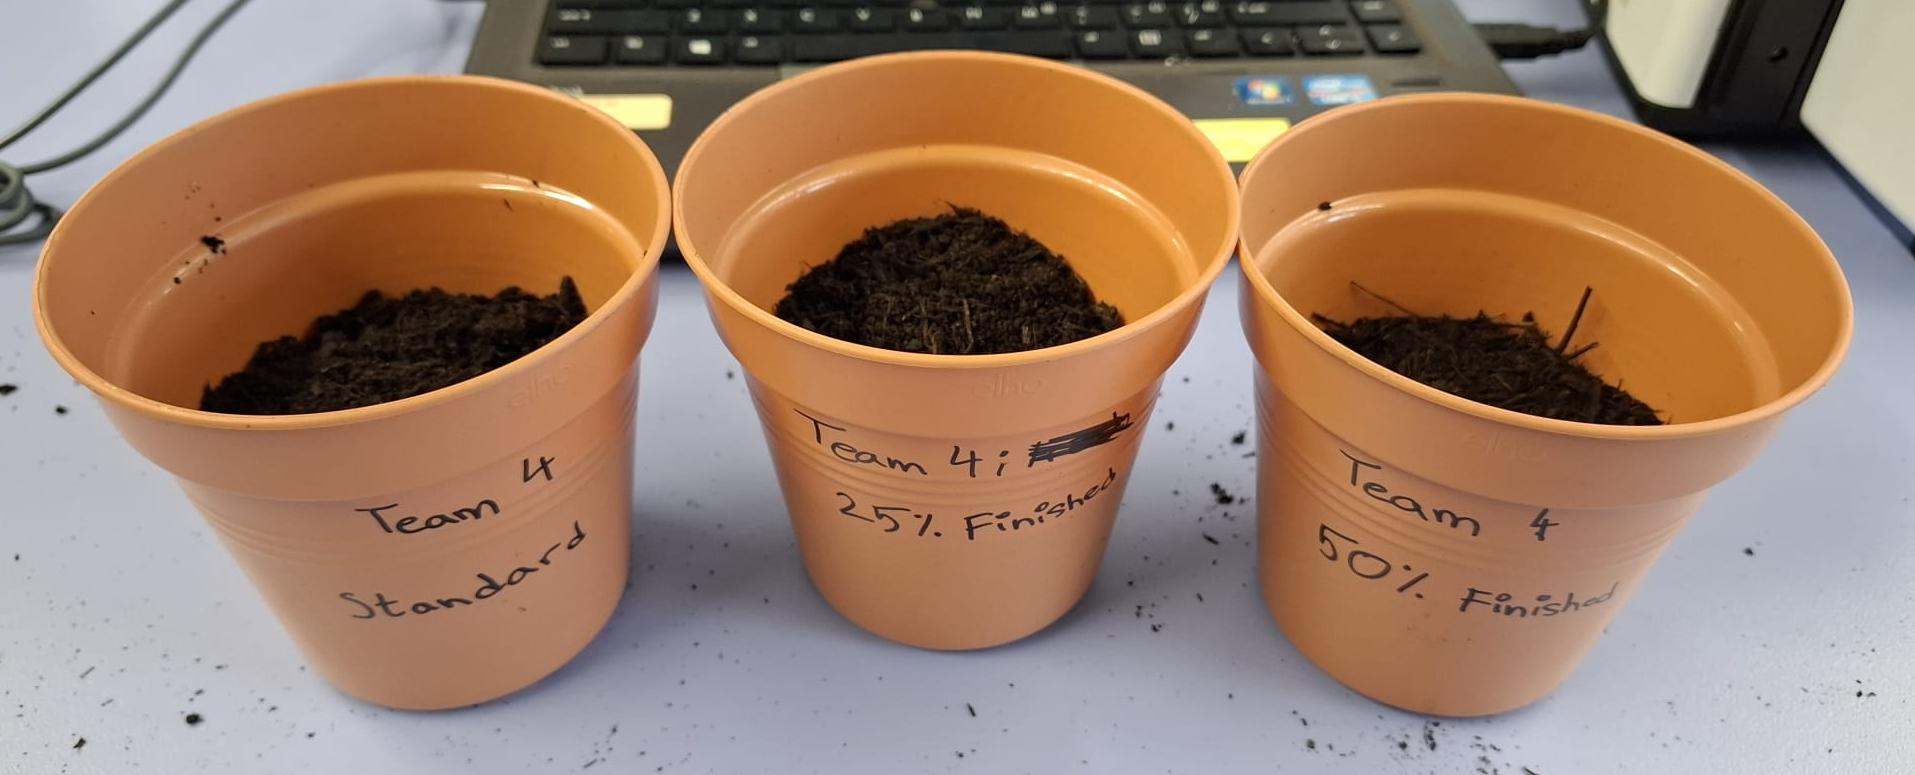
\includegraphics[width=\textwidth]{media/pots.jpeg}
        \caption{Triplet of compost inside the pots}
    \end{minipage}
\end{figure}
\vspace*{.5cm}

\newpage
\subsection{Results}
\subsubsection{Preliminary parameters}
We collected three samples: Fresh, Finished, and Standard, and 
valuated them based on several characteristics, including pH, color,
texture, odor, foreign objects, and moisture content. Each sample had
distinct features, which helped us assess their condition and quality. 

\renewcommand{\arraystretch}{1.5}
\begin{table*}[ht!]
    \centering \vspace{.3cm}
    \caption{Results of preliminary parameters}
    \hspace*{-.3cm}
    \begin{tabular}{|c|c|c|c|c|c|c|}
        \hline
        \textbf{Sample name} & \textbf{pH} & \textbf{Color} & \textbf{Texture} & \textbf{Odor} & \textbf{Foreign objects} & \textbf{Moisture fist test}\\
        \hline
        Fresh & 9 & Light brown & Coarse & Smells ammonia & -- & 30\% humidity\\
        \hline                                                                   
        \multirow{2}{*}{Finished} & \multirow{2}{*}{8} & \multirow{2}{*}{Dark brown} & \multirow{2}{*}{Fine} & \multirow{2}{*}{Smells ammonia} & Sticks and & \multirow{2}{*}{20\% humidity} \\
                                  &   &            &      &                & plastic particles & \\
        \hline
        Standard & 7 & Darkest brown & Clumpy & Smells earthy & -- & 30\% humidity\\
        \hline
    \end{tabular}
\end{table*}
\phantom{} \vspace*{-.2cm}

\subsubsection{Fresh, Finished and Standard compost}
Three samples were collected, and their raw unit weight was evaluated.
The mass of the empty cylinder was measured in grams, with a value of
168.24 g. The mass of the filled cylinder for each sample was then
measured, obtaining values in liters. The volume of each sample was
also measured in milliliters. Using these measurements, the density
results were calculated in both [kg/L] and [kg/m$^3$] using the formulas:

$\displaystyle \text{Density} \left[kg/L\right] = \frac{\text{Mass of filled cylinder}\ [g] - \text{Mass of empty cylinder}\ [g]}{\text{Volume of sample}\ [mL]}$

$\displaystyle \text{Density} \left[kg/m^3\right] = \text{Density} \left[kg/L\right] \cdot 1000 \left[L/m^3\right]$

The average values provided insight into the consistency of the raw
unit weight across the different samples.


\subsubsection{Fresh compost}
\renewcommand{\arraystretch}{1.5}
\begin{table*}[ht!]
    \centering \vspace{.3cm}
    \caption{Results of raw unit weight in three different samples of fresh compost}
    \begin{tabular}{|c|c|c|c|c|}
        \hline
        \textbf{Sample} & \textbf{1} & \textbf{2} & \textbf{3} & \textbf{Average}\\
        \hline
        {\textbf{Mass of the empty}} & \multicolumn{4}{c|}{\multirow{2}{*}{168.24}}\\
        \textbf{cylinder in [g]} & \multicolumn{4}{c|}{}\\
        \hline
        \textbf{Mass of the filled} & \multirow{2}{*}{120.88} & \multirow{2}{*}{112.20} & \multirow{2}{*}{108.71} & \multirow{2}{*}{113.93}\\
        \textbf{cylinder [g]} & & & &\\
        \hline
        \textbf{Volume of the} & \multirow{2}{*}{340} & \multirow{2}{*}{330} & \multirow{2}{*}{390} & \multirow{2}{*}{353.33}\\
        \textbf{sample in [mL]} & & & &\\
        \hline
        \textbf{Result in [kg/L]} & 0.356 & 0.34 & 0.279 & 0.325\\
        \hline
        \textbf{Result in [kg/m$^3$]} & 356 & 340 & 279 & 325\\
        \hline
    \end{tabular}
\end{table*}

\newpage
\subsubsection{Finished compost}
\renewcommand{\arraystretch}{1.5}
\begin{table*}[ht!]
    \centering \vspace{.3cm}
    \caption{Results of raw unit weight in three different samples of finished compost}
    \begin{tabular}{|c|c|c|c|c|}
        \hline
        \textbf{Sample} & \textbf{1} & \textbf{2} & \textbf{3} & \textbf{Average}\\
        \hline
        {\textbf{Mass of the empty}} & \multicolumn{4}{c|}{\multirow{2}{*}{168.24}}\\
        \textbf{cylinder in [g]} & \multicolumn{4}{c|}{}\\
        \hline
        \textbf{Mass of the filled} & \multirow{2}{*}{214.54} & \multirow{2}{*}{202.91} & \multirow{2}{*}{202.68} & \multirow{2}{*}{206.71}\\
        \textbf{cylinder [g]} & & & &\\
        \hline
        \textbf{Volume of the} & \multirow{2}{*}{375} & \multirow{2}{*}{370} & \multirow{2}{*}{380} & \multirow{2}{*}{375}\\
        \textbf{sample in [mL]} & & & &\\
        \hline
        \textbf{Result in [kg/L]} & 0.572 & 0.548 & 0.533 & 0.551\\
        \hline
        \textbf{Result in [kg/m$^3$]} & 572 & 548 & 533 & 551\\
        \hline
    \end{tabular}
\end{table*}

\subsubsection{Standard compost}
\renewcommand{\arraystretch}{1.5}
\begin{table*}[ht!]
    \centering \vspace{.3cm}
    \caption{Results of raw unit weight in three different samples of standard compost}
    \begin{tabular}{|c|c|c|c|c|}
        \hline
        \textbf{Sample} & \textbf{1} & \textbf{2} & \textbf{3} & \textbf{Average}\\
        \hline
        {\textbf{Mass of the empty}} & \multicolumn{4}{c|}{\multirow{2}{*}{168.24}}\\
        \textbf{cylinder in [g]} & \multicolumn{4}{c|}{}\\
        \hline
        \textbf{Mass of the filled} & \multirow{2}{*}{222.95} & \multirow{2}{*}{228.44} & \multirow{2}{*}{212.74} & \multirow{2}{*}{221.38}\\
        \textbf{cylinder [g]} & & & &\\
        \hline
        \textbf{Volume of the} & \multirow{2}{*}{355} & \multirow{2}{*}{370} & \multirow{2}{*}{360} & \multirow{2}{*}{361.67}\\
        \textbf{sample in [mL]} & & & &\\
        \hline
        \textbf{Result in [kg/L]} & 0.628 & 0.617 & 0.591 & 0.612\\
        \hline
        \textbf{Result in [kg/m$^3$]} & 628 & 617 & 591 & 612\\
        \hline
    \end{tabular}
\end{table*}

\newpage
\subsection{Experiment results}
\renewcommand{\arraystretch}{1.5}
\begin{table*}[ht!]
    \centering \vspace{.3cm}
    \caption{Experiment results}
    \begin{tabular}{|c|l|l|l|l|l|l|}
        \hline
        \textbf{Group 4} & \textbf{E0} & \textbf{E0} & \textbf{E25} & \textbf{E25} & \textbf{E50} & \textbf{E50} \\
        \hline
        n$^{\circ}$ germinated seeds & 12 & 13 & 11 & 12 & 11 & 10\\
        \hline
        weight (g) & 1.672 & 1.882 & 0.997 & 1.294 & 1.058 & 1.105\\
        \hline
    \end{tabular}
\end{table*}

\vspace*{2cm}
\cfig{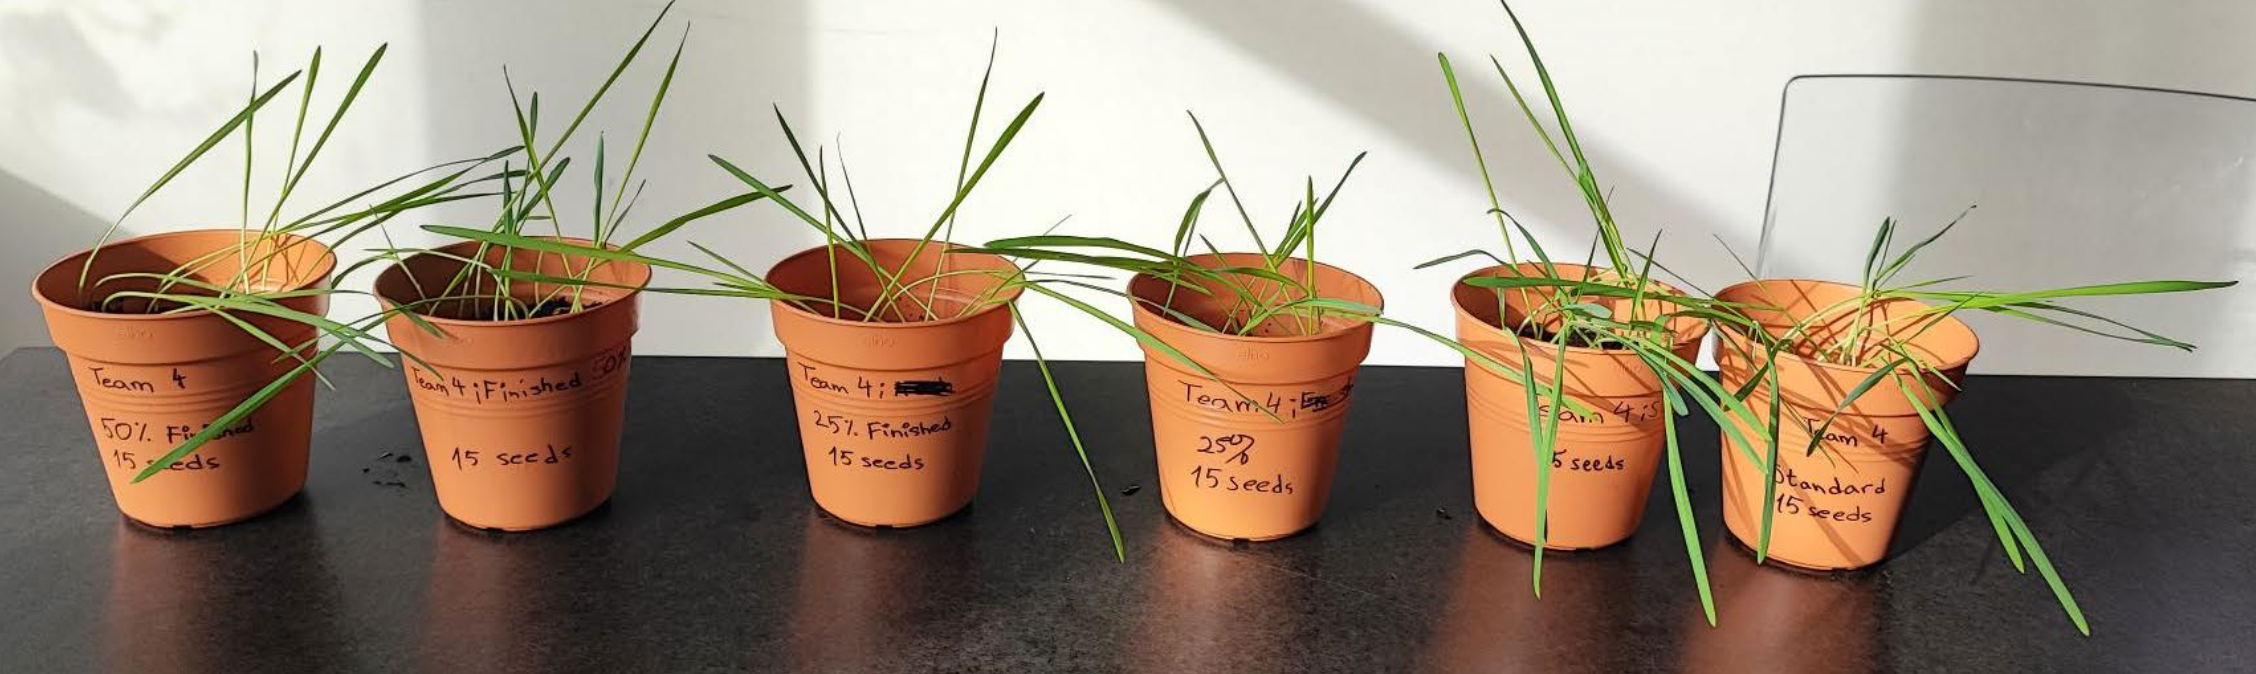
\includegraphics[width=.9\textwidth]{media/plants-results.png}}

\newpage
\subsection{Discussion}
Interpret the results, discussing and answering the questions.

\subsubsection{Results discussion}

\subsubsection{Questions}
\begin{enumerate}
    \item What is the difference between raw unit weight and bulk density? Discuss your
        results based on the laboratory experiment.

        \textbf{R:\\}
        Raw unit weight is the density given by the division of the mass of the compost
        over the volume of the compost. The bulk unit is the density given by the division
        of the mass of the compost over the volume of the container.

    \item How can the pH affect the compost?
    
        \textbf{R:\\}
        The more acidic the soil is, the more inactive the bacteria are, and this bring
        plants to not grow properly. Vice versa for the basicity.\\
        Compost microorganisms operate best under neutral to acidic conditions, with pH's
        in the range of 5.5 to 8. During the initial stages of decomposition, organic
        acids are formed. The acidic conditions are favourable for growth of fungi and
        breakdown of lignin and cellulose \parencite{cornell}.

    \item What is the impact of immature compost on plant growth, and how can this be
        assessed in the lab?

        \textbf{R:\\}
        Plants will not grow properly if the nitrogen cycle is not working. Indeed, it is
        generally accepted that compost produced with substrates rich in nitrogen will
        have a better fertilizing effect, compared to other compost whose substrates are
        mainly woody. Likewise, immature compost will have a repressive effect on seed
        germination and plant growth \parencite{tamakloe2021}.\\
        In the lab, we can do the germination test and for immature compost you have
        standard growth.

    \item How do you calculate the bulk density of compost, and why is this measurement
        important in the composting process?

        \textbf{R:\\}
        Divide the mass of the compost by the volume of the container. Bulk density
        provides an overall indication for the physical and aeration conditions of a
        composting mass \parencite{bulk_density}.

    \item What would be the environmental impact if fresh compost is added in the
        plantations/agriculture or when the recommended percentage of compost mixture
        is not followed?

        \textbf{R:\\}
            Using fresh or excessive compost can release methane, impair growth through
            nitrogen depletion, and cause nutrient leaching, leading to water contamination.

\end{enumerate}

\subsection{Conclusion}
Summarize the key findings and their implications.

\newpage
\setlength{\bibitemsep}{1.2\baselineskip}

\printbibliography

\listoftables

\listoffigures

\section*{Declarations about AI tools}
\begin{itemize}
    \item ``\textit{ChatGPT-4 with canvas}'' was used as a tool to enhance vocabulary.\\
        {\color{darkgray!95}{\textit{All original sentences come from our individual thoughts and were refined with
        the support of this tool.}}}\\
        \url{https://chatgpt.com/}
    \item ``DeepL'' was used as a translator.\\
        \url{https://www.deepl.com}
\end{itemize}






\end{document}
